The following sources of uncertainties are considere for the data-driven multi-jet estimation in the $\tau_{had}\tau_{had}$ channel, described in Section~\ref{subsec:HadHadmultijet}:

\begin{itemize}
\item Statistical uncertainties on the FFs (compare~\Cref{fig:hadhad_fake_factors});
\item Statistical uncertainties on the TFs (compare~\Cref{fig:hadhad_transfer_factors});
\item Difference between SS and OS regions;
\item Background subtraction.
\end{itemize}

The size of the STT FFs uncertainty is about 10\% per fake factor bin. The
largest variation resulting from varying a single fake factor results in a
0.2\% normalisation uncertainty on the total multi-jet fake background. This is due to
the small fraction of STT events selected by the analysis.

Similarly, the size of the 1-prong DTT FF uncertainties is less than 5\% per FF
bin. The largest variation from a single FF bin results in a 0.6\% normalisation
uncertainty. The size of the 3-prong DTT FFs uncertainties is less than 10\% per
FF bin and the largest impact results in a 0.4\% normalisation uncertainty.

The analysis is insensitive to the variations in the individual FFs bins as the
fake template statistical uncertainty is larger than the measurement uncertainty
of the fake factor measurement. Thus, the number of variations are reduced
combining the variations of all fake factor bins by adding them in quadrature.
The statistical uncertainties on the FFs results in this way in a flat
uncertainty of 1.4\% on the normalisation.

The effect of the statistical uncertainties of the TFs on the multi-jet
normalisation is shown in Table~\ref{sec:systs:tab:systematics_multijet_TFs}.
Independent uncertainties are added for 1- and 3-prong anti-\tauhad where the
anti-\tauhad is the leading and subleading \tauhad candidate. Shape
effects are propagated to the fit. This uncertainty targets the extrapolation of
the fake factors from the 1-tag measurement region to the 2-tag application
region.

\begin{table}
\centering
\small
\begin{tabular}{|c|c|}
\hline
Source & Impact on normalisation\\
\hline
TF (1-prong, Lead. $\tau_{had}$) & 3.3\%\\
TF (1-prong, Subl. $\tau_{had}$) & 3.3\%\\
TF (3-prong, Lead. $\tau_{had}$) & 2.0\%\\
TF (3-prong, Subl. $\tau_{had}$) & 1.9\%\\
\hline
Total & 5.5\%\\
\hline
\end{tabular}
\caption{Effect of TFs statistical uncertainties, parametrised in \tauhad prong
  and whether the anti-\tauhad is the leading or subleading \tauhad-candidate,
  on multi-jet normalisation in the di-Higgs $bb\tau_{had}\tau_{had}$ channel. }
\label{sec:systs:tab:systematics_multijet_TFs}
\end{table}

Differences between the SS regions where the FFs are calculated and the OS
region where they are applied are estimated by comparing the nominal 1 -btag FFs
to FFs derived in the 1 b-tag OS region where additional cuts are applied to
reduce the large contamination of non-fake backgrounds in the OS ID-region (fake
purity before the cuts is about 50\%, after the cuts is about 76\%):
\begin{itemize}
\item $m_{\tau\tau}^{MMC}>110$ GeV (to reduce Z+jets);
\item $E_{T}^{miss}/\sigma_{E_T^{miss}}<3$ (to reduce $t\bar{t}$).
\end{itemize}
The FFs are found to be similar in the OS and SS regions, as shown in
Figures~\ref{fig:systs_HadHad_multijet_OSSSDTT1P}-~\ref{fig:systs_HadHad_multijet_OSSSSTT}.

\begin{figure}[h]
  \centering

  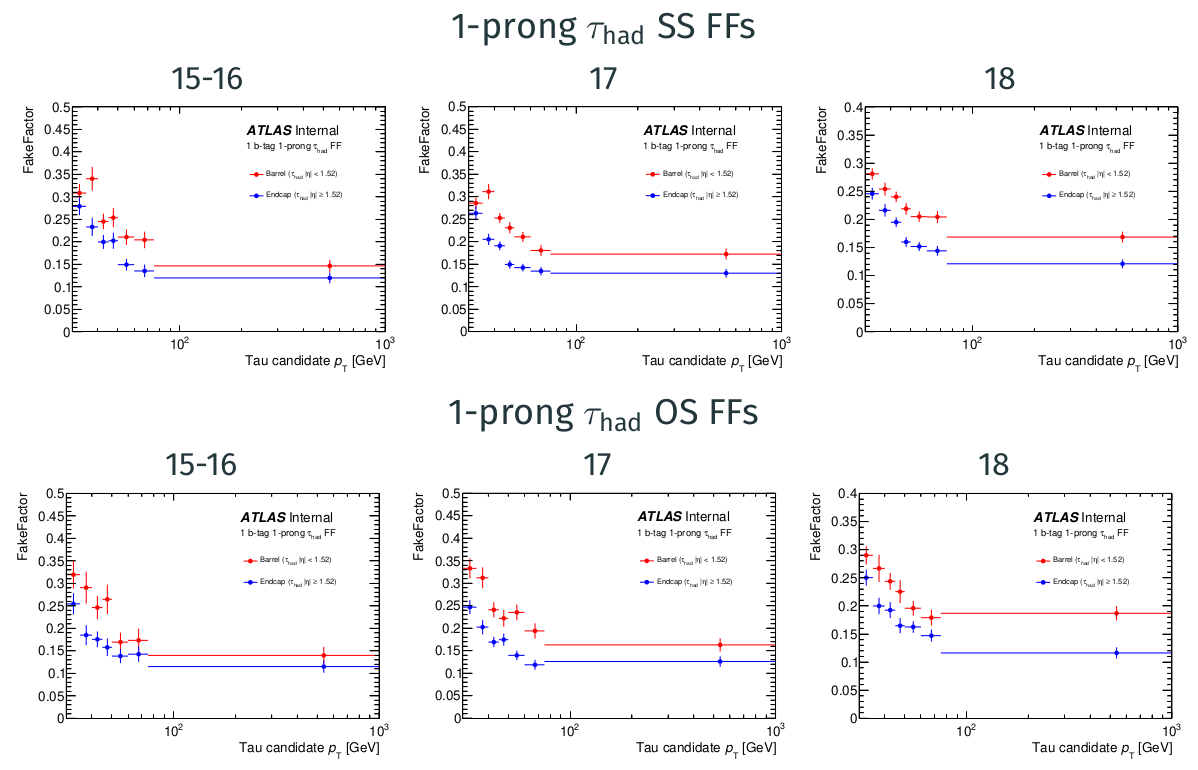
\includegraphics[width=.85\textwidth]{figures/systs/hadhad_multijet/OSSS_DTT1P}
  \caption{FFs in SS (up) and OS (down) regions for DTT 1-prong.}

  \label{fig:systs_HadHad_multijet_OSSSDTT1P}
\end{figure}

\begin{figure}[h]
  \centering

  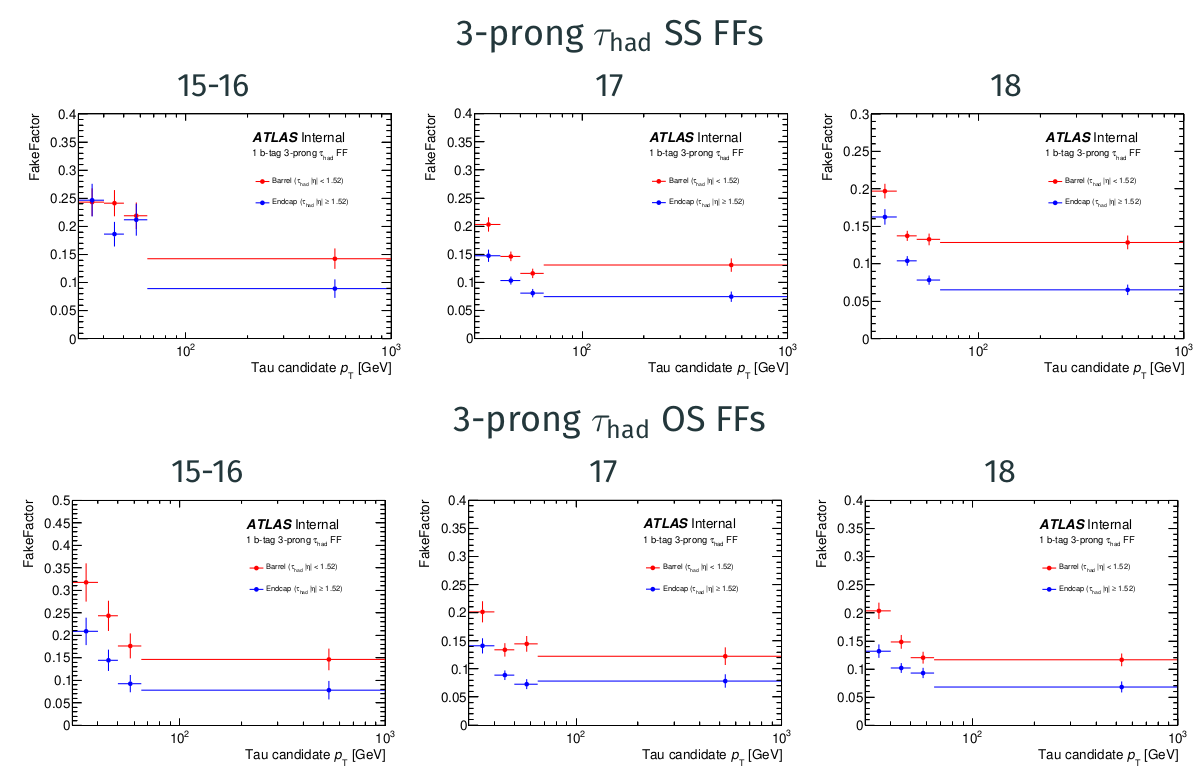
\includegraphics[width=.85\textwidth]{figures/systs/hadhad_multijet/OSSS_DTT3P}
  \caption{FFs in SS (up) and OS (down) regions for DTT 3-prongs.}

  \label{fig:systs_HadHad_multijet_OSSSDTT3P}
\end{figure}

\begin{figure}[h]
  \centering

  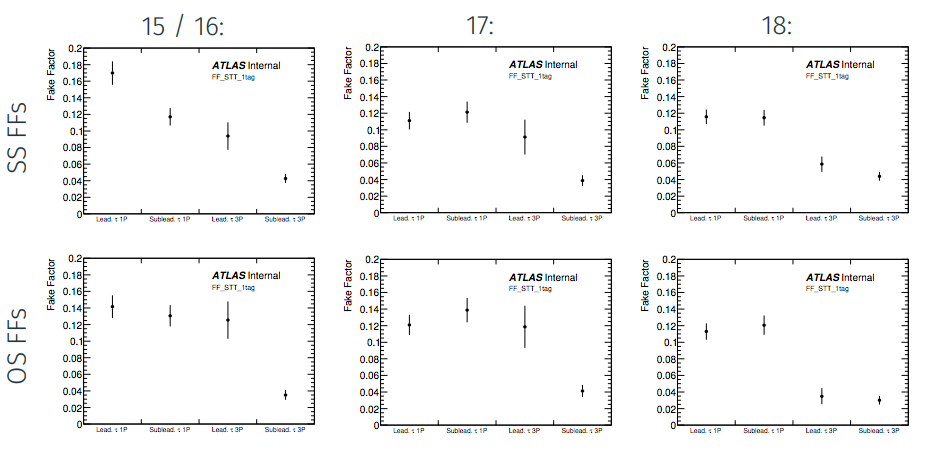
\includegraphics[width=.85\textwidth]{figures/systs/hadhad_multijet/OSSS_STT}
  \caption{FFs in SS (up) and OS (down) regions for STT.}

  \label{fig:systs_HadHad_multijet_OSSSSTT}
\end{figure}

The ratio of the OS to SS FFs is applied as uncertainty and it is resulting in a
2.2\% uncertainty on the multi-jet normalisation. The shape impact of this
uncertainty is propagated to the fit.

For the subtraction of non-multi-jet backgrounds in the regions used for the
data-driven multi-jet estimation, there is a relatively small subtraction in the
1 b-tag SS CRs where the FFs are derived but a large subtraction of about 50\%
(from \ttbar) in the 2 b-tags OS Anti-ID region where the FFs are applied to
obtain the multi-jet template, as shown in
Appendix~\ref{subsec:appendix_bkg_multijetj_HadHad}. The uncertainty of the
subtraction on the fake factors is neglected since the subtraction uncertainty
will be dominated by the large relative subtraction in the 2 b-tag OS Anti-ID
region.

The uncertainty due to the subtraction of non-multi-jet backgrounds in
the 2-tag OS Anti-ID region is split into the origin of the dominant
backgrounds that are being subtracted: true \tauhad \ttbar, fake
\tauhad \ttbar, and other (predominantely V+jets / single-top).

The subtraction uncertainty of true \tauhad \ttbar is estimated by
comparing the nominal prediction of \ttbar (true \tauhad) with the
uncertainty prescriptions for the \ttbar-process by PMG in the 2-tag
OS Anti-ID region. The breakdown of uncertainties is depicted
in~\Cref{tab:systematics_multijet_hh_ttbar_subtraction}. The fake
estimate variations are provided by varying the subtraction of true
\tauhad \ttbar by the total uncertainty
($\substack{+16.8 \% \\ -18.6 \%}$) in the 2-tag OS Anti-ID region
when estimating the multi-jet fake background. The impact on the
normalization of the fake template after true \tauhad \ttbar
subtraction is $\pm 2.41 \%$.

\begin{table}[htbp]
  \centering
  \begin{tabular}{lr}
    \toprule
    Source & Uncertainty \\
    \midrule
    ME & $\pm 6.0 \%$ \\[0.3em]
    PS & $\pm 11.0 \%$ \\[0.3em]
    $\mu_\text{R}$ & $\substack{+9.9 \% \\ -9.4 \%}$ \\[0.3em]
    $\mu_\text{F}$ & $\substack{+2.8 \% \\ -2.2 \%}$ \\[0.3em]
    ISR & $\substack{+0.53 \% \\ -0.68 \%}$ \\[0.3em]
    FSR & $\substack{+5.4 \% \\ -10.0 \%}$ \\
    \midrule
    Total & $\substack{+16.8 \% \\ -18.6 \%}$ \\
    \bottomrule
  \end{tabular}
  \caption{Uncertainty on true \tauhad \ttbar in the 2-tag OS Anti-ID region.}
  \label{tab:systematics_multijet_hh_ttbar_subtraction}
\end{table}

The subtraction uncertainty of fake \tauhad \ttbar is estimated using
the dedicated scale factor measurement introduced
in~\Cref{sssec:ttbar_fake_sf_antiid}. The variance of the scale factor
measurement is dominated by the leading eigenvariations due to the
large correlations of the scale factors measured in the Anti-ID
region. Therefore, only the leading eigenvariation for every offline
\tauhad identification and trigger setup is propagated to the fake
estimate. Moreover, due to the limited set of experimental
uncertainties used for the scale factor measurement in the Anti-ID
region, the full difference of the scale factors to 1 is taken as an
additional uncertainty and propagated to the fake estimate. A
breakdown of the normalization impact is shown
in~\Cref{tab:systematics_multijet_hh_fake_ttbar_subtraction}. The
shape impact of the individual NPs is propagated to the fit.

\begin{table}[htbp]
  \centering
  \begin{tabular}{lr}
    \toprule
    Nuisance Parameter & Impact on multi-jet fake yield \\
    \midrule
    \texttt{TTBAR\_FAKESF\_ANTITAU\_OFFL\_EIGEN0} & $\pm 0.09 \%$ \\
    \texttt{TTBAR\_FAKESF\_ANTITAU\_TAU25\_EIGEN0} & $\pm 3.97 \%$ \\
    \texttt{TTBAR\_FAKESF\_ANTITAU\_TAU25EF\_EIGEN0} & $\pm 2.05 \%$ \\
    \texttt{TTBAR\_FAKESF\_ANTITAU\_TAU25RNN\_EIGEN0} & $\pm 4.71 \%$ \\
    \texttt{TTBAR\_FAKESF\_ANTITAU\_DIFF} & $\pm 2.00 \%$ \\
    \midrule
    Total & $\pm 6.80 \%$ \\
    \bottomrule
  \end{tabular}
  \caption{Normalization impact of fake \tauhad subtraction uncertainties on the fake estimate.}
  \label{tab:systematics_multijet_hh_fake_ttbar_subtraction}
\end{table}

Due to the small relative subtraction of other backgrounds, which are
predominantely composed of V+jets and single-top events, a
conservative estimate of the subtraction uncertainty is defined by
varying the subtraction of these backgrounds up and down by $50
\%$. This has an impact of $\pm 5.22 \%$ on the final multi-jet fake
estimate. The shape uncertainty of the subtraction is propagated to
the fit.

The total uncertainty on the normalisation of the multi-jet background is 10.7\%.

Plots showing the shape effect of these systematics on the MVA distributions are shown in Appendix~\ref{subsec:appendix_systs_multijetsysts_hadhad}.
